\documentclass[10pt]{article}

\usepackage[english]{babel} 
\usepackage[T1]{fontenc}
\usepackage{cite, url,color} % Citation numbers being automatically sorted and properly "compressed/ranged". 
%\usepackage{pgfplots}
\usepackage{graphics,amsfonts}
\usepackage[pdftex]{graphicx}
\usepackage[cmex10]{amsmath}
% Also, note that the amsmath package sets \interdisplaylinepenalty to 10000
% thus preventing page breaks from occurring within multiline equations. Use:
 \interdisplaylinepenalty=2500
% after loading amsmath to restore such page breaks as IEEEtran.cls normally does.

\usepackage[utf8]{inputenc}
%% Useful packages for creation of two-column and more complex figures

% Compact lists
\usepackage{enumitem}


\usepackage{array}
% http://www.ctan.org/tex-archive/macros/latex/required/tools/
\usepackage{mdwmath}
\usepackage{mdwtab}
%mdwtab.sty	-- A complete ground-up rewrite of LaTeX's `tabular' and  `array' environments.  Has lots of advantages over
%		   the standard version, and over the version in `array.sty'.
% *** SUBFIGURE PACKAGES ***
\usepackage[tight,footnotesize]{subfigure}

\usepackage[top=2cm, bottom=2cm, right=1.6cm,left=1.6cm]{geometry}
\usepackage{indentfirst}
\usepackage{float}

\usepackage{times}
%\usepackage[active]{srcltx}
\graphicspath{{./figure/}}

\setlength\parindent{0pt}
\linespread{1}

\def\C#1{\mathcal{#1}}

\renewcommand{\phi}{\varphi}
% COMMON OPERATORS
\newcommand{\floor}[1]{{\left\lfloor #1\right\rfloor}}
\newcommand{\ceil}[1]{{\left\lceil #1\right\rceil}}
\newcommand{\E}[1]{\mathop{\rm E}\nolimits\left[#1\right]} % Expectation
\newcommand{\pr}[1]{\Pr\left[ #1 \right]}
\renewcommand{\P}[1]{\mathrm{P}\left[ #1 \right]}
\newcommand{\mbb}{\mathbb}
\newcommand{\mrr}{\mathrm}
\newcommand{\mmin}[1]{{\min\left\{#1\right\}}}
\newcommand{\mmax}[1]{{\max\left\{#1\right\}}}
\newcommand{\id}[1]{\mathbf{1}\(#1\)} % Unit function  
\newcommand{\Heav}[1]{\mathcal{H}\left(#1\right)} % Heaviside function
\newcommand{\eps}{\varepsilon}
\newcommand{\rect}[1]{\mathrm{rect}\!\left(#1\right)}
\newcommand{\sinc}[1]{\mathrm{sinc}\!\left(#1\right)}
\newcommand{\bin}[2]{{\left(\begin{array}{c}#1\\#2\end{array}\right)}}

\newcommand{\me}[2]{\left[ {#1} \right]_{(#2)}} % Submatrix \me{P}{i,j} produces [P]_{i,j} and denotes the element in the i-th row and j-th column of P
\newcommand{\vv}[1]{\left[ {#1} \right]} % Submatrix \vv{a,b,c} produces [a,b,c]

\newcommand{\Set}[1]{{\C #1}} 
\newcommand{\Setd}[2]{\Set{#1}=\left\{#2\right\}}  % Set definition: \Set{S}{0,1,2} produces S={01,2,} where S is in mathcal 

\newcommand{\mat}[1]{{\hbox{\textbf{#1}}}}
\newcommand{\ei}[1]{{\mat{e}_{#1}}}   % all zero vector except in the $#1$-th element which is one
\newcommand{\ind}[1]{\mathbf{\chi}\left\{#1\right\}} % Indicator function \ind{A}=1 if A is true, \ind{A}=0 otherwise. 

% FORMATTING
\newcommand{\ie}{i.e.,\,}
\newcommand{\eg}{e.g.,\,}
\newcommand{\columnbreak}{\vfill\eject} % Column break

% REFERENCES
\newcommand{\Fig}[1]{Fig.~\ref{#1}}
\newcommand{\eq}[1]{(\ref{#1})}
\newcommand{\Tab}[1]{Tab.~\ref{#1}}
\newcommand{\Sec}[1]{Sec.~\ref{#1}}

% COMMENTS/REVISIONS
\newcommand{\AZ}[1]{\textit{\color{magenta}#1}} 

% Compact title; retain the template's 10 pt text and prescribed margins.
\makeatletter
\renewcommand{\@maketitle}{%
  \begin{center}
  {\Large\@title\par}\vskip 0.6em
  {\normalsize\@author\par}
  \end{center}}
\makeatother

\begin{document}
\title{Network modeling -- AY 2026/2027\\
Homework 1 -- Modeling Zoom video uplink traffic}
\author{Alessandro Vulcu -- ID 2185190\\University of Padua}
\date{}
\maketitle
\vspace{-1.4em}
\begin{abstract}
I analyze one outbound UDP flow from a Zoom meeting between a PC and an iPad.
Packets occur in tight clusters, which a Poisson source fails to reproduce.
An empirical batch-renewal model captures packet-gap and size distributions and
matches the mean rate on a held-out segment. It does not reproduce the observed
correlation of traffic over longer time scales.
\end{abstract}
\vspace{-0.6em}

\section{Measurement and sample selection}
I captured Zoom traffic with Wireshark on the PC's Ethernet interface
\texttt{enp5s0}; the iPad was a second participant on the same LAN.
The experiment progressed through idle/muted operation, a connected meeting with
media off, microphone-only speech and silence, camera-on speech, and camera off
again. These phase durations were approximate: the stopwatch ran for about ten
minutes, so I do not treat the planned durations as exact boundaries.

The video-related flow was identified by switching the PC camera off and on and
observing its traffic decrease and recover. Its endpoints were
\texttt{192.168.3.7:42613} and \texttt{206.247.58.75:8801}.
I selected only the PC-to-server direction using
\begin{center}
\small\texttt{udp.stream == 0 \&\& ip.src == 192.168.3.7 \&\& frame.number > 32864}.
\end{center}
\vspace{-0.5em}
The filter retains 34,319 packets spanning 615.08 s. I set $t=0$ at the first
selected packet (431.2223 s into the raw capture), not at the stopwatch start.
The rate rises near $t=260$ s and falls near $t=578$ s (Fig.~\ref{fig:timeline}).
I therefore select the interior camera-on interval $[270,570)$ s: 32,136 packets,
300 s, and 862.50 kbit/s. I fit the model on the first 180 s and reserve the last
120 s for validation.
No selected packet is truncated. Packet sizes are \texttt{frame.len} in bytes,
including captured Ethernet headers, not encoded media payload.

\begin{figure}[ht]
\centering
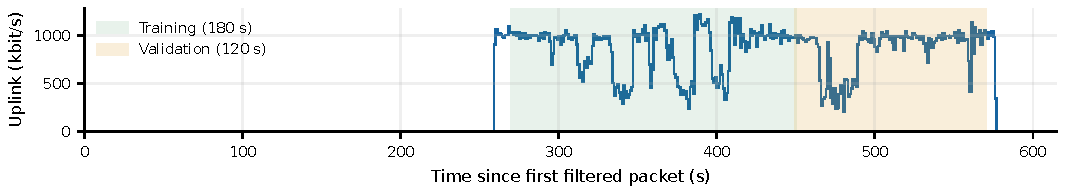
\includegraphics[width=\textwidth]{zoom_phase_timeline.pdf}
\vspace{-1em}
\caption{One-second uplink rate and the selected training and validation intervals.
Camera transitions are inferred from traffic; audio-only phase boundaries are not resolved in this flow.}
\label{fig:timeline}
\end{figure}
\vspace{-1.2em}

\section{Source model}
In the training segment, packet gaps have mean 9.162 ms, median 5.38 $\mu$s,
and coefficient of variation 1.711; 63.17\% are at most 1 ms.
I first fit a Poisson baseline: $A_i\sim\mathrm{Exp}(109.145\,\mathrm{s}^{-1})$,
$B_i\equiv1$, and independent packet sizes sampled from the training empirical
distribution. Its exponential gaps cannot represent the concentration near zero.

Following Lessons 3--4, I model the bursty VBR source with a marked and weighted
renewal process, augmented with packet offsets.
Consecutive packets separated by at most $\delta=1$ ms
belong to the same cluster. These clusters are defined by packet timing; they do
not identify codec frames. Let $\tau_i$ be a cluster's first timestamp, $B_i$ its packet count,
$U_{i,k}$ its packet offsets, and $W_{i,k}=8L_{i,k}$ its weights in bits.
Each complete training cycle stores the joint tuple
\[
 C_i=(D_i,B_i,\{U_{i,k},W_{i,k}\}_{k=1}^{B_i}),
 \qquad D_i=\tau_{i+1}-\tau_i.
\]
I exclude the boundary clusters, leaving 7,233 cycles. To generate a trace,
I draw cycles independently and uniformly from this empirical distribution,
emit packets at $\tau_i+U_{i,k}$, then advance by $D_i$.
Thus batch inter-arrivals satisfy $A_{i+1}=D_i$; weights, counts and offsets
remain dependent within a sampled cycle. Offsets prevent artificial zero packet gaps.
The fitted means are $E[D]=24.881$ ms and $E[B]=2.716$ packets, with predicted rate
$E[\sum_k W_{i,k}]/E[D]=865.95$ kbit/s. Thresholds of 0.5 and 3 ms give mean
batch sizes 2.707 and 2.774, close to the value at 1 ms.

\clearpage
\begin{figure}[H]
\centering
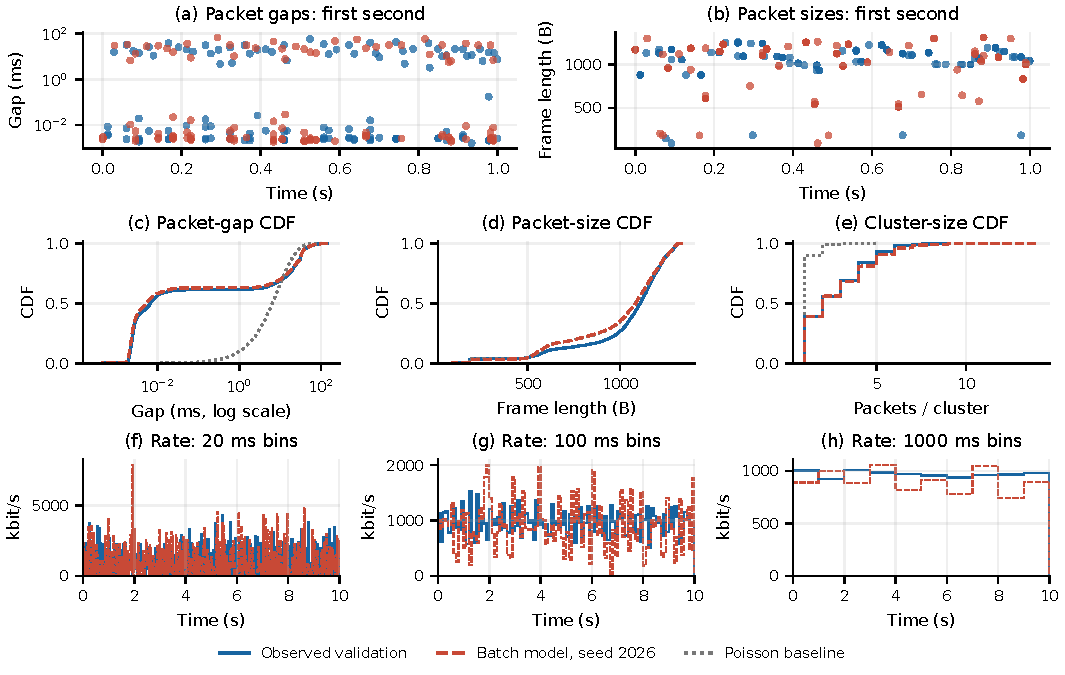
\includegraphics[width=0.96\textwidth]{zoom_model_comparison.pdf}
\vspace{-1em}
\caption{Held-out observations and independent 120 s simulations (seed 2026).
Scatterplots show the first second; CDFs use the full traces; rate plots show the
first ten seconds. Cluster sizes in (e) use the same 1 ms rule for every trace.
Synthetic events are not expected to align with observed events.}
\label{fig:comparison}
\end{figure}
\vspace{-1.3em}
\section{Results}
\vspace{-0.5em}
\begin{center}
\small
\setlength{\tabcolsep}{9pt}
\begin{tabular}{lrrr}
\hline
120 s validation comparison & Observed & Poisson & Batch model\\
\hline
Packet count & 12,491 & 12,927 & 13,102\\
Mean frame length (B) & 1,029.57 & 989.97 & 990.38\\
Mean rate (kbit/s) & 857.35 & 853.16 & 865.06\\
Packet-gap CDF distance & --- & 0.611 & 0.050\\
Count Fano factor, 100 ms bins & 1.115 & 0.995 & 2.475\\
Lag-1 count correlation, 1 s bins & 0.684 & 0.151 & 0.049\\
\hline
\end{tabular}
\end{center}
\vspace{-0.6em}
Both simulations use training data only and stop at 120 s; packet counts are
stochastic, not forced to match observations. The batch simulation's mean rate
is 0.90\% above validation. Across 30 seeds (2026--2055), its mean rate is
864.30 kbit/s; the empirical 5th--95th percentile range is 847.42--879.97 kbit/s.
Figure~\ref{fig:comparison} shows that the batch model preserves short packet gaps
much better than Poisson: the maximum absolute empirical CDF difference falls
from 0.611 to 0.050. This is a descriptive distance, not an independence-based
significance test. The size-CDF distance is 0.089 for the batch model, reflecting
some shift in sizes between training and validation.

\vspace{-0.6em}
\section{Discussion}
The batch model captures local clustering and average load, but overestimates
100 ms count variability and loses the strong correlation between successive
one-second counts. Independent cycle sampling discards ordering across clusters;
it therefore misses slow activity or adaptation changes. A state-dependent or
block model could address this limitation.
This single run covers one video-related UDP flow, not all Zoom traffic or
separately identified audio. Phase boundaries are inferred and payloads are
encrypted. The model describes packets observed at the host capture interface,
not the encoder's internal generation times or a universal Zoom traffic law.
Controlled camera changes alone do not provide enough cycles to estimate an
On--Off sojourn-time model. Course basis: Lesson 3, \emph{Network abstraction and
traffic source models}; Lesson 4, \emph{Traffic source models}.

\end{document}
